\section{Wetter und Klima}
\begin{frame}
	% TODO: Wetter vs. Klimadaten Dortmund: zB Osterwetter vs klassisches Niederschlags-Temperatur-Diagramm anfertigen
	
	% TODO: Daten dazu beim dwd oder bei der Stadt Dortmund Stichwort Opendata -Weather bzw. Witterung
	
	%TODO: Campuswetter der TU NICHT nutzbar, da urheberrechtlich geschützt
	\frametitle{Wetter und Klima}
	\begin{columns}[onlytextwidth]
		\begin{column}[t]{0.49\linewidth}
			\textbf{Wetter}\\
			\textit{\enquote{ist der physikalische Zustand der Atmosphäre an einem bestimmten Ort zu einem \alert{bestimmten Zeitpunkt} oder in einem kurzen Zeitraum.}}
			\begin{itemize}
				\item Gekennzeichnet durch Ist-Werte von Temperatur, Luftfeuchtigkeit, Niederschlag, ...
				\item Ist was wir täglich mit unseren Sinnen erleben
			\end{itemize}
		\end{column}%
		\begin{column}[t]{0.49\linewidth}
			\textbf{Klima}\\
			\textit{\enquote{ist der mittlere Zustand der Atmosphäre an einem bestimmten Ort über einen \alert{längeren Zeitraum.}}}
			\begin{itemize}
				\item Gekennzeichnet durch statistische Mittelwerte (circa 30 Jahre) der selben Größen
				\item Ist entscheidend für die Entwicklung der Ökosysteme
			\end{itemize}
		\end{column}%
	\end{columns}
	\pause
	\bigskip
	\begin{center}
		Das (durchschnittliche) Wetter macht das Klima, \\
		das Klima bestimmt das (wahrscheinliche) Wetter.
	\end{center}
	
	\vfill
	\tiny{Zitate von \url{https://www.umweltbundesamt.de/service/uba-fragen/was-ist-eigentlich-klima}}
	
\end{frame}

\begin{frame}
	\frametitle{Klima}
	\begin{itemize}
		\item Auch definiert als Zustand des klimatischen Systems %WMO
		\item Betrachtung verschiedener Parameter wie Temperatur, Niederschlag, Windgeschwindigkeiten % WMO
		\item Betrachtet werden u.a. Mittelwert, Abweichung und Wahrscheinlichkeit des Auftretens extremer Ereignisse z.B. Dürren %M.Latif, Klimawandel und Klimadynamik S. 11
		\item Aus dem Griechischen: \textit{klinein} $\equiv$ neigen $\rightarrow$ Neigung der Erdachse
	\end{itemize}

	%TODO: Abbildung für Neigung der Erde (Sommer/Winter auf der Nordhalbkugel) und Position der Sonne
\end{frame}

\begin{frame}
	\frametitle{Klima - Neigung der Erdachse}
	\begin{figure}
		\centering
		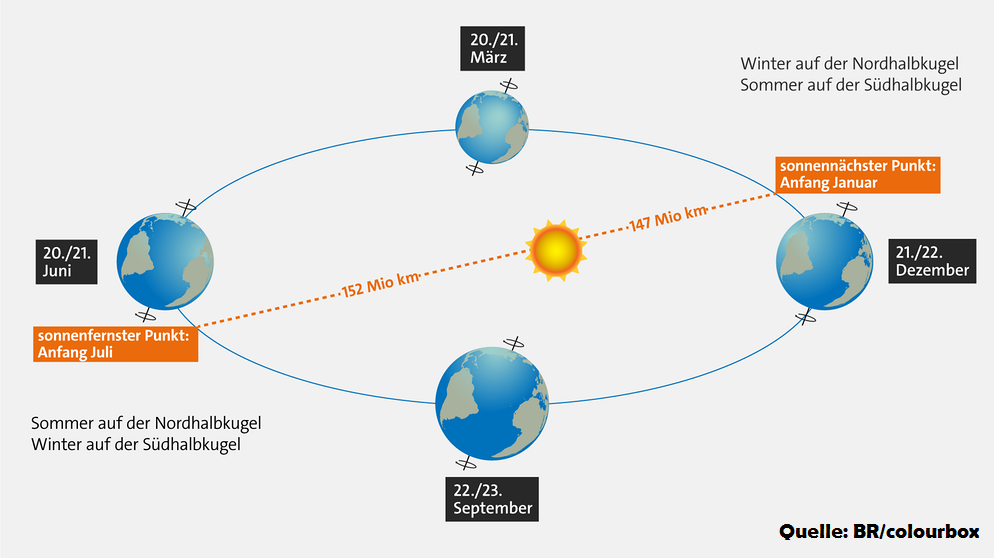
\includegraphics[width=0.5\linewidth]{bilder/Erdumlaufbahn_DWD.png}
		\caption{Neigung der Erdachse als Ursache für die Jahreszeiten, Quelle: Deutscher Wetterdienst}
	\end{figure}

	\begin{itemize}
		\item Die Neigung der Erde ist entscheidend für die Sonneneinstrahlung auf der Erde
		\item [$\rightarrow$] und damit verantwortlich für die Jahreszeiten und das Klima auf der Nord und Südhalbkugel
	\end{itemize}
\end{frame}

\begin{frame}
\frametitle{Klima - Eiszeitzyklen}
\begin{figure}
	\centering
	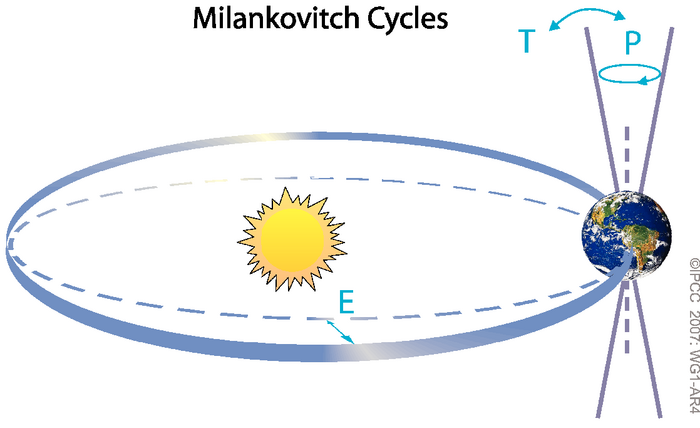
\includegraphics{bilder/milankovitch_IPCC2007_AR4.png}
	\caption{Milankovitch-Zyklen: Periodische Änderungen der Erdbahnparameter, Quelle: IPCC 2007, WG1, Kapitel 6}
\end{figure}
\begin{itemize}
	\item E: Veränderung der Ausdehnungsrichtung der Erdbahn (Exzentrizität)% - aktuell: 0,017 perfekter Kreis bei 0, leicht elliptisch bei 0,05
	\item P: Schwankung der Erde um die Erdachse (Präzession) % da die Erde keine perfekte Kugel ist
	\item T: Veränderung des Neigungswinkels der Erdachse (eng. tilt)
	\item[$\rightarrow$] verursachen Eiszeitzyklen, sowie deren Warm- und Kaltphasen
	\item[$\rightarrow$] langfristiger Einfluss auf das Klima
\end{itemize}
\end{frame}


\begin{frame}
	\frametitle{Klimaänderung}
	\begin{block}{Klimaänderung}
		Erkennbare (messbare) Änderung Klimas über einen gewissen Zeitraum (z.B. 30 Jahre) %M.Latif Klimawandel und Klimadynamik S. 13
		Spürbar durch Änderung atmosphärischer Größen wie der Temperatur
	\end{block}

	\only<2->{
	\begin{figure}
		\centering
		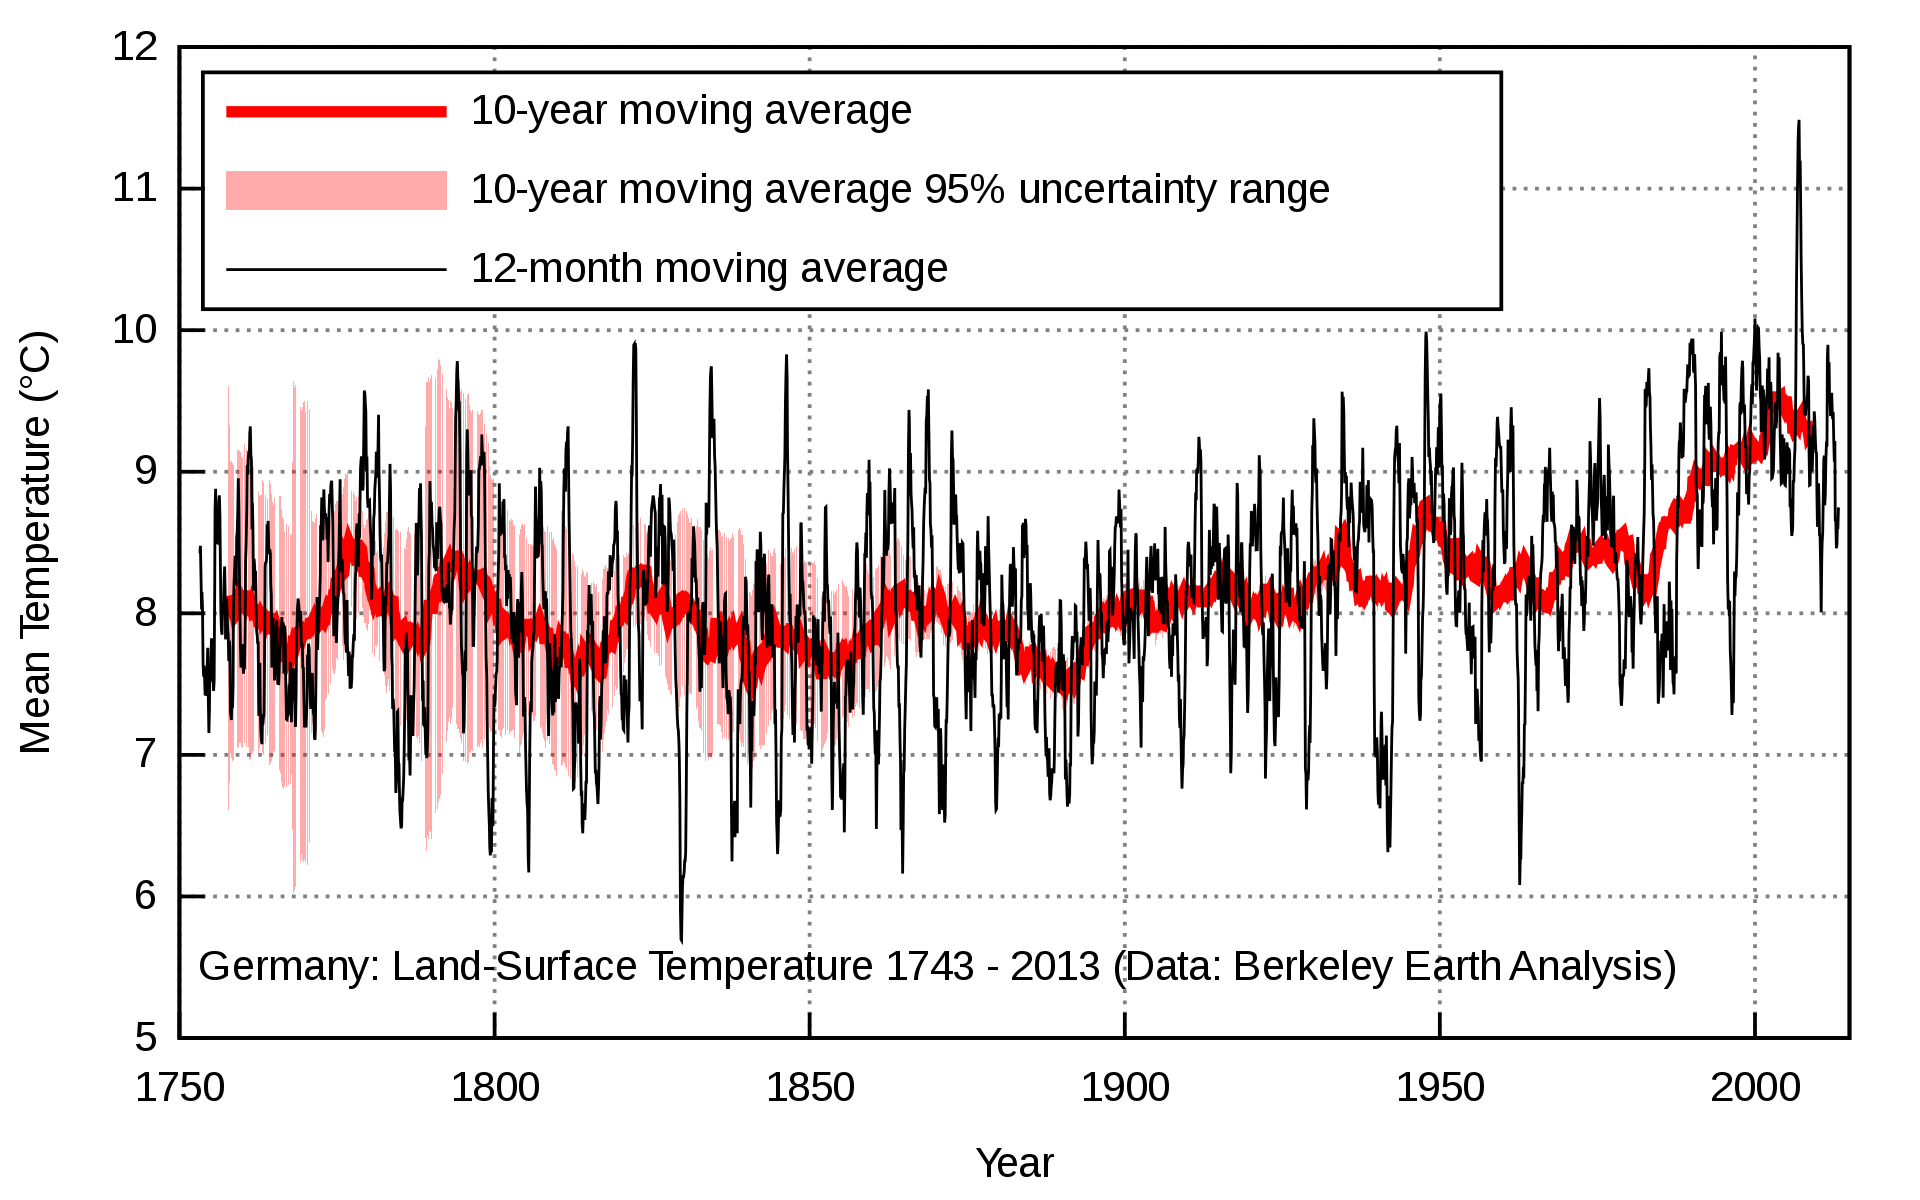
\includegraphics[width=0.6\linewidth]{bilder/Temp_Deutschland_1743-2013_Berkley_Wiki.png}
		\caption{Entwicklung der mittleren Jahrestemperaturen in Deutschland, Quelle: Wikipedia, Daten: Berkeley Earth Surface Temperature Project}
	\end{figure}
	}
% Die Abbildung zeigt die mittleren Temperaturen in Deutschland pro Jahr von 1743 bis 2013
% Wenn man sich jetzt so einen 30-Jahre zeitraum anschaut, ist die Änderung des Klima-Parameters Oberflächentemperatur deutlich erkennbar

\end{frame}

\begin{frame}
	\frametitle{Klimavorhersagen} %TODO
	\begin{itemize}
		\item Die statistischen Eigenschaften des Wetters lassen sich längerfristig Vorhersagen.
		\item[$\rightarrow$] Jahreszeiten, Monsunregen, etc.. %TODO: Bedingungen dafür in  Kapitel 3.3 aus M.Latif nachlesen
		\item Atmosphärische Änderungen im Kontext des Erdsystems
		\item [$\rightarrow$] Hydrosphäre, Kryosphäre, Biospähre, Pedosphäre und Lithosphäre % Stichwort Wechselwirkungen
	\end{itemize}
\end{frame}
